\chapter{Análise Bibliográfica sobre Testes automatizados de software, por Jônatas Gomes Barbosa da Silva\label{chap:bibliometria:titofrota}}

\section{Planejamento do estudo}

\textit{Automação de teste}, área do campo da \textit{engenharia de software}, é o uso de software para controlar a execução do teste de software, a comparação dos resultados esperados com os resultados reais, a configuração das pré-condições de teste e outras funções de controle e relatório de teste. 

A automação dos testes vem do grande custo de tempo e recursos financeiros para a realização de testes manuais. Dessa forma, os testes manuais estão sendo substituídos pelos automáticos, com o custo da profundidade dos testes, visto que alguns efeitos colaterais de determinadas interações e entradas não conseguem ser testadas da mesma forma que nos testes manuais.

Partindo dos pontos acima, as questões que nortearam a pesquisa foram:
\begin{itemize}
    \item Quais são as técnicas mais utilizadas \textit{testes automatizados}?
    \item Quais os esforços aplicados na melhoria das técnicas existentes?
    \item Qual tem sido a aderência na implementação de novas técnicas?
\end{itemize}

\subsection{Uso do Bibliometrix e Biblioshiny}
Serão usadas a ferramenta e o \textit{workflow} proposto pelos autores do pacote Bibliometrix, conforme indica a figura ~\ref{fig:bibliometrix:workflow}.

\subsection{Limitações} O exercício relatado foi feito em 3 horas e meia, utilizando a base de dados Web of Science (WoS).


\section{Coleta de dados\label{MASSA:coleta}}

A coleta de dados feita usando a base Web of Science (WoS) no dia 10 de janeiro de 2022, acessado por meio do Portal de Periódicos da CAPES.

Foi usada a \textit{query} de busca ilustrada loog abaixo:

test driven automation
test driven
graph convolutional networks

\subsection{Explicação para os termos de busca usados\label{sec:titofrota:query}}

A busca utilizando estes termos se deve pela lógica de tentar encontrar artigos voltados para o tema de grafos, com foco em redes neurais e inteligência artificial. Os termos podem aparecer no título, no abstract ou nas palavras chave.

O termo grafo se refere às buscas voltadas para esta estrutura de dados. Já seus adjetivos como redes neurais e inteligência artificial foram usados para entender aplicações mais específicas.

Foram obtidos mais de 15 mil registros com a \textit{query} utilizada. Na exportação, foi utilizado o formato de arquivo de texto sem formatação, com os 29 campos disponíveis.

\section{Análise dos dados}

\subsection{Filtragem de registros}

Para não poluir demais os gráficos, foi feita uma filtragem com os 2000 artigos mais relevantes do tema.

\subsection{Análise descritiva do \textit{dataset} }

A seguir, é feita uma análise bibliométrica descritiva do \textit{dataset} utilizando a função \texttt{biblioAnalysis} do Bibliometrix, que realiza diversos cálculos para levantar as taxas apresentadas.

As informações mais gerais sobre o \textit{dataset} são as seguintes:
\begin{description}
    \item [\textit{Timespan}] Os artigos filtrados foram publicados entre 1966 e 2022.
    \item [\textit{Sources (Journals, Books, etc)}] São 1024 fontes de informação que publicaram os artigos recuperados no \textit{dataset}.
    \item [\textit{Average years from publication}] A média do tempo de publicação dos artigos no \textit{dataset} é de 5.89 anos.
    \item [\textit{Average citations per documents}] Cada artigo no \textit{dataset} foi citado, em média 7.44 vezes.
    \item [\textit{Average citations per year per doc}] Após publicado, cada um dos artigos foi citado, em média, 1.35 vezes por ano.
    \item [\textit{References}] O \textit{dataset} contém 49.429 referências citadas.
    \item [\textit{Keywords Plus (ID)}] 1444 distintas palavras-chave do tipo Keywords Plus (ID) foram encontradas no \textit{dataset}.
    \item [\textit{Author's Keywords (DE)}] 4276 distintas palavras-chave indicadas pelos autores foram encontradas no \textit{dataset} .
    \item [\textit{Authors}] 6.017 distintos nomes de autores foram encontrados no \textit{dataset} .
    \item [\textit{Author Appearances}] Os autores foram encontrados 8.036 vezes, como autores de artigos.
    \item [\textit{Authors of single-authored documents}] 121 autores editaram artigos individualmente, isso é, sem co-autores.
    \item [\textit{Authors of multi-authored documents}] 5.896 autores editaram artigos com um ou mais co-autores.
    \item [\textit{Single-authored documents}] 134 documentos foram escritos por um único autor, e os restantes foram elaborados em co-autoria.
    \item [\textit{Documents per Author}] Cada autor publicou em média 0.332 artigos.
    \item [\textit{Authors per Document}] 3.01 autores por documento.
    \item [\textit{Co-Authors per Documents}] 4.02 co-autores por documento.
    \item [\textit{Collaboration Index}] 3.16 indíces de colaboração.
\end{description}

\subsection{Evolução da Produção Científica}

\begin{figure}
    \centering
    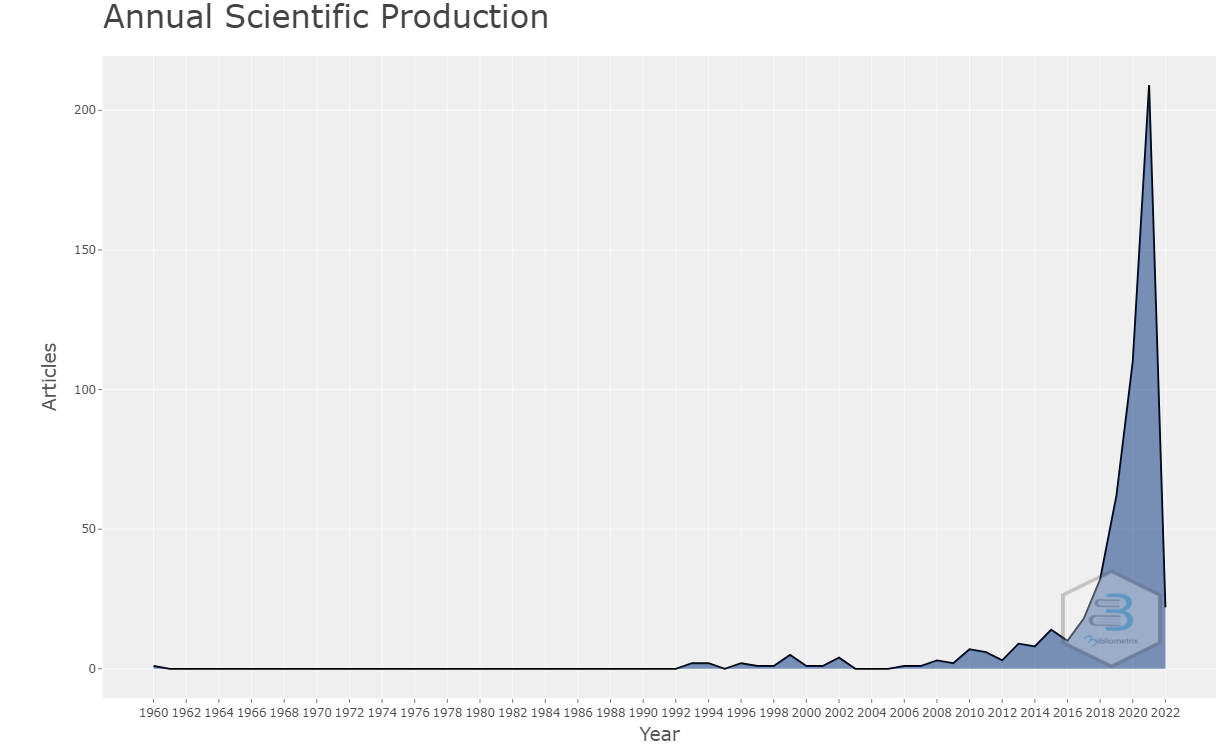
\includegraphics[width=1\textwidth]{experiments/titofrota/PesquisaBibliometrica/Deepfakes/annual-plot.png}
    \caption{Evolução da produção científica no \textit{dataset}}
    \label{fig:evol:anual:DEEPFAKES@titofrota}
\end{figure}

A figura \ref{fig:evol:anual:DEEPFAKES@titofrota} representa a evolução em produção científica mundial a respeito do tema, de acordo com o \textit{dataset}. Houve um crescimento a notável a partir do ano de 2020, atingindo o pico em 2021. 
É perceptível que no \textit{dataset} ainda há artigos não relacionados ao tema analisado.

O \textit{Annual Growth Rate} do \textit{dataset} é de 12,62\%, que é um valor alto comparado a média de crescimento da comunidade científica como um todo.

\subsection{Interpretação do Crescimento} a taxa de crescimento do \textit{dataset} demonstra que o tema tem chamado muita atenção nos últimos anos, provavelmente devido aos escândalos envolvendo pessoas públicas e os \textit{deepfakes}.

\subsection{Evolução das Citações}

\begin{figure}
    \centering
    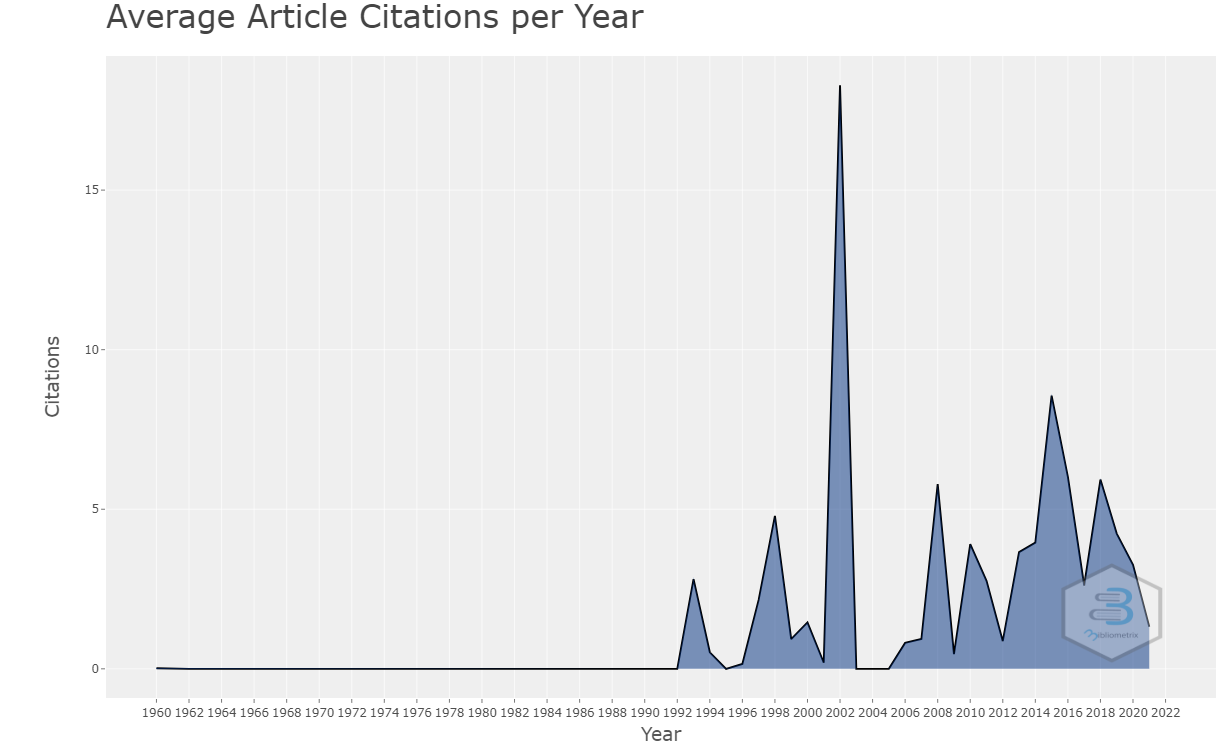
\includegraphics[angle=0,width=1\textwidth]{experiments/titofrota/PesquisaBibliometrica/Deepfakes/citations-year-plot.png}
    \caption{Evolução das citações ao \textit{dataset}.}
    \label{fig:evol:anual:citacoes:DEEPFAKES@titofrota}
\end{figure}

A figura \ref{fig:evol:anual:citacoes:DEEPFAKES@titofrota} apresenta a evolução da média de citações aos artigos do \textit{dataset}. Não há muita estabilidade na média anual de citações, até mesmo nos anos mais recentes.

\subsection{Interpretação das Citações}
Embora a taxa de crescimento de publicações anuais seja alta, ainda há instabilidade no que diz respeito a média de citações. Demonstrando que o tema ainda é um tanto prematuro, necessitando de mais atenção pelos cientistas.

\subsection{\textit{Three-Field Plots (Sankey diagram)}}

As \textit{Three-Field Plots (Sankey diagram)} (plotagens do tipo ``Três Campos'') correlacionam três conjuntos de atributos em busca das afinidades encontradas no \textit{dataset}. Assim, são demonstrados os principais fluxos entre diferentes conjuntos.

\begin{figure}
    \centering
    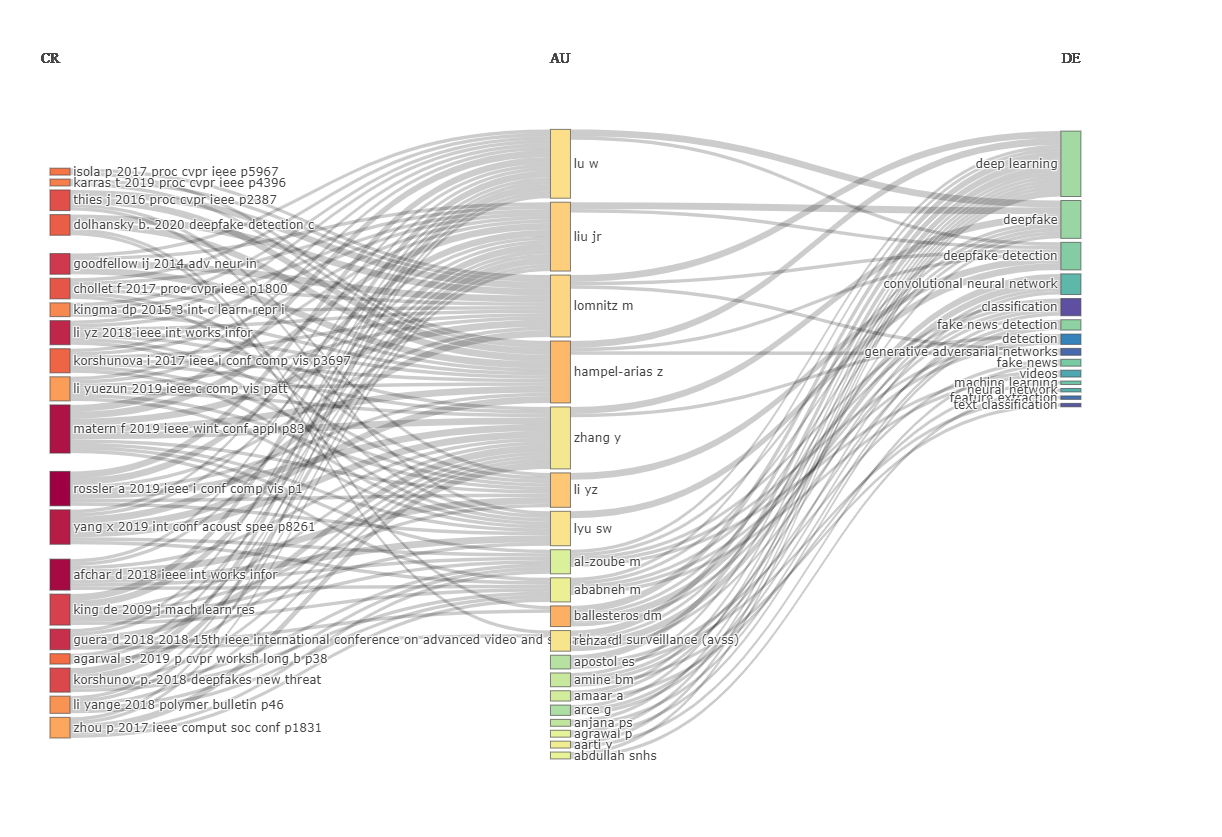
\includegraphics[width=1\textwidth]{experiments/titofrota/PesquisaBibliometrica/Deepfakes/ThreeFieldPlot.png}
    \caption{Plotagem ``Três Campos'' (Sankey plot) do \textit{dataset}: 20 Autores, Citações e 14 Palavras-Chave mais proeminentes.}
    \label{fig:DEEPFAKES@titofrota:ThreeFieldPlot}
\end{figure}

A figura \ref{fig:DEEPFAKES@titofrota:ThreeFieldPlot} apresenta a plotagem do tipo ``Três Campos'' realizada no \textit{dataset}, vinculando, ao centro, os 20 Autores mais proeminentes (AU), à esquerda, as 20 Citações mais frequentes (CR - Cited Records), e à direita, as 14 Palavras-Chave mais frequentes empregadas pelos autores.

\subsection{Interpretação da figura \ref{fig:DEEPFAKES@titofrota:ThreeFieldPlot}}
A maioria dos autores mais relevantes apresentados na plotagem são, aparentemente, de origem oriental, mais especificamente chinesa. Além disso, uma quantidade razoável dos artigos surgiram em universidades da China. O que sugere o avanço e a preocupação do oriente a respeito do tema analisado.

É possível observar nas palavras-chave que há bastante interesse na detecção de \textit{deepfakes}, apresentam-se os termos \textbf{deepfake detection}, \textbf{fake news detection} e \textbf{detection}. Os resultados sugerem que há interesse em remediar os impactos que os conteúdos criados através de algoritmos de \textit{deep learning} podem causar à sociedade.

\section{Refinamento da Coleta de Dados}

Após a análise do \textit{dataset}, foi possível notar que há a presença de artigos que não estão relacionados ao tema. A observação indica a necessidade de uma nova busca, visando a exclusão de artigos não relacionados ao desenvolvimento de \textit{deepfakes}.

Ao analisar a rede de co-ocorrência de palavras aplicada ao \textit{dataset}, foram identificadas algumas palavras no cluster que não correspondem ao assunto trabalhado. Assim, surgiu uma nova \textit{query} para levantar artigos mais apurados e relevantes.

\begin{figure}[htp]
    \centering
    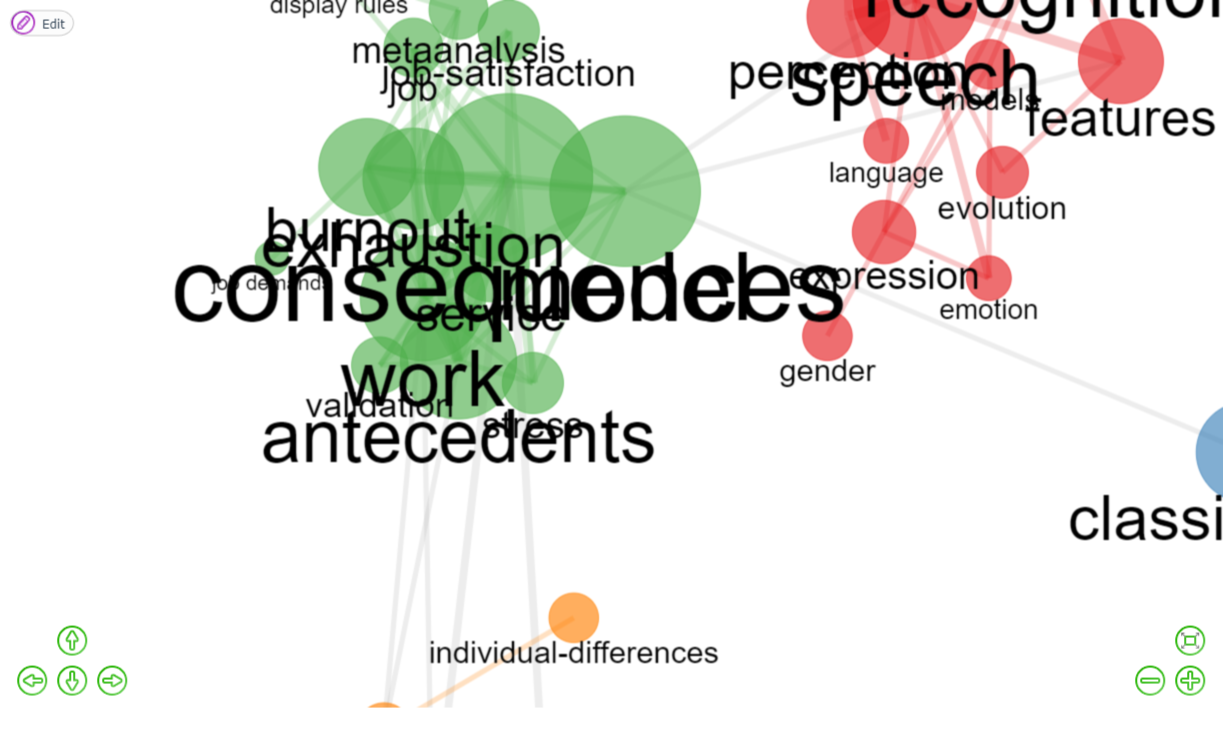
\includegraphics[width=0.6\textwidth]{experiments/titofrota/PesquisaBibliometrica/Deepfakes/co-ocurrence.png}
    \caption{Rede de co-ocorrência de palavras aplicada ao \textit{dataset}.}
    \label{fig:DEEPFAKES@titofrota:redecoocorrencia}
\end{figure}

A nova \textit{query} leva em conta novos termos e a busca foi feita nas publicações entre 2017 (quando o termo \textit{deepfake} surgiu) e 2022.

\lstinputlisting[numbers=left,basicstyle=\normalsize\ttfamily,caption={Query refinada de busca sobre Deepfakes.}]
{experiments/titofrota/PesquisaBibliometrica/Deepfakes/new-query.txt}


Além das justificativas para os termos usados entre as linhas 1 a 9, já descritas em \ref{MASSA:query},  justifica-se na listagem \ref{query20220203}, a inclusão da cláusula \textit{not (
 adsoption or molecular -dynamics or force -field
 or in -vitro or nanopartic* or in -vivo
 or aqueous -solution or protein or surface)}, entre as linhas 10 e 13 da \query, pois elas irão remover artigos não se enquadram no escopo da busca desejada, por usarem uma ou mais desses termos no título, resumo ou palavras-chave do artigo.
 
 Foram incluídas cláusulas como \textbf{deep-fake} e \textbf{face-swap*} com o intuito de encontrar mais conteúdos relacionados ao tema. Além disso, foram adicionadas novas cláusulas negadas para filtrar melhor os resultados, evitando que artigos médicos ou relacionados à outros temas façam parte do novo \textit{dataset}.
 
Usando a nova \textit{} de busca, foram recuperados 284 documentos. Sendo assim, aproximadamente 749 registros não se enquadravam na necessidade de busca.
Uma nova análise dos dados recuperados é apresentada a seguir.

\section{Nova Análise dos Dados}

\subsection{Nova filtragem de registros}

São aplicados dois filtros aos 284 documentos recuperados:
\begin{itemize}
    \item Remoção dos registros de documentos que não são artigos \textit{full paper}, isso é, artigos completos publicados em revistas;
    \item Remoção dos registros de artigos científicos que não fazem parte do \textit{core} da bibliografa, segundo a Lei de Bradford.
\end{itemize}

Após a filtragem, foram obtidos apenas 79 registros, que correspondem ao novo \textit{dataset}.
08
\subsection{Análise descritiva do \textit{dataset} refinado}

\begin{table}[]
    \centering
\csvautotabular[separator=semicolon
%,filter not strcmp={\csvcolii}{}
]{experiments/titofrota/PesquisaBibliometrica/Deepfakes/main-info.csv}
    \caption{Principais dados descritivos do dataset refinado.}
    \label{tab:DEEPFAKE:Main}
\end{table}

Logo, de acordo com a tabela \ref{tab:DEEPFAKE:Main}, é possível notar que entre 2017 e 2022 houveram 240 artigos publicados em 94 revistas diferentes.